\section{Methods and Methodology}

\begin{figure}[!h]
    \centering
        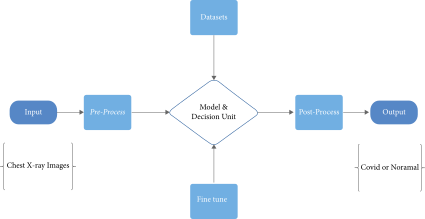
\includegraphics{assets/block.png}
    \caption{Block Diagram~\cite{Uddin2021} of the Proposed System}
\end{figure}

\subsection{Data Collection/Input:}

The data set is collected from different sources. We have proposed a framework that can effectively detect COVID-19 cases by evaluating the chest x-ray images. The image data are collected from different websites such as Radiopedia.org and Figure1.com. The random images are studied and divided into Normal image and Covid image. This data set is further converted into training and testing with the split of 70\% data for training of proposed deep learning model and 30\% data for testing purpose. 

\subsection{Data pre-processing }

Due to inconsistency of the dataset, the X-ray images are of different sizes. So, the all the images are converted to the same size. Also, splitting dataset process and data augmentation technique comes under data pre-processing. Final input to the proposed model is prepared. 
